\documentclass{standalone}
\usepackage{tikz}
\usepackage{ctex,siunitx}
\usepackage{tkz-euclide}
\usepackage{amsmath}
\usetikzlibrary{patterns, calc}
\usetikzlibrary {decorations.pathmorphing, decorations.pathreplacing, decorations.shapes,}
\begin{document}
\small
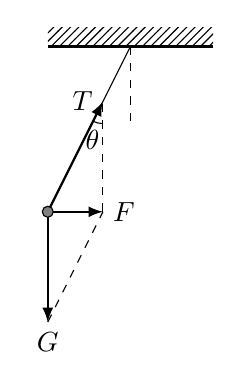
\begin{tikzpicture}[>=latex,scale=0.7]
  \fill [pattern = north east lines] (-1.5,0) rectangle (1.5, .34);
  \draw[thick](-1.5,0)--(1.5,0);
  \draw[dashed](0,0)--(0,-1.5) ;
  \draw[dashed](-.5,-3)--(-.5,-1) ;
  \draw[dashed](-1.5,-5)--(-.5,-3) ;
  \draw (0,0)--(-1.5,-3) ;
  \draw [->, thick] (-1.5,-3)--(-.5,-1) node [left]{$T$};
  \draw [->, thick] (-1.5,-3)--(-.5,-3) node [right]{$F$};
  \draw [->, thick] (-1.5,-3)--(-1.5,-5) node [below]{$G$};
  \draw (-.5,-1-.4) arc(-90:-118:.4) node [below]{$\theta$};
  \draw [fill=gray] (-1.5,-3)  circle [radius=.1];
\end{tikzpicture}
\end{document}